\section{Durchführung}
\label{sec:Durchführung}
Für die Durchführung dieses Versuches wird grundlegend ein Laser, ein drehbarer Spiegel und ein schwenkbares Photoelement benötigt. Damit Information aus dem Photoelement 
gezogen werden kann, wird dieses über ein Amperemeter ausgewertet. Der schematische Aufbau des Versuches wird in \autoref{fig:Aufbau1} dargestellt. Da der verwendete Laser 
kein polarisiertes Licht emittiert, muss zwischen dem Laser und dem Spiegel noch ein \textit{Polarisationsfilter} plaziert werden. 

\begin{figure}
    \centering
    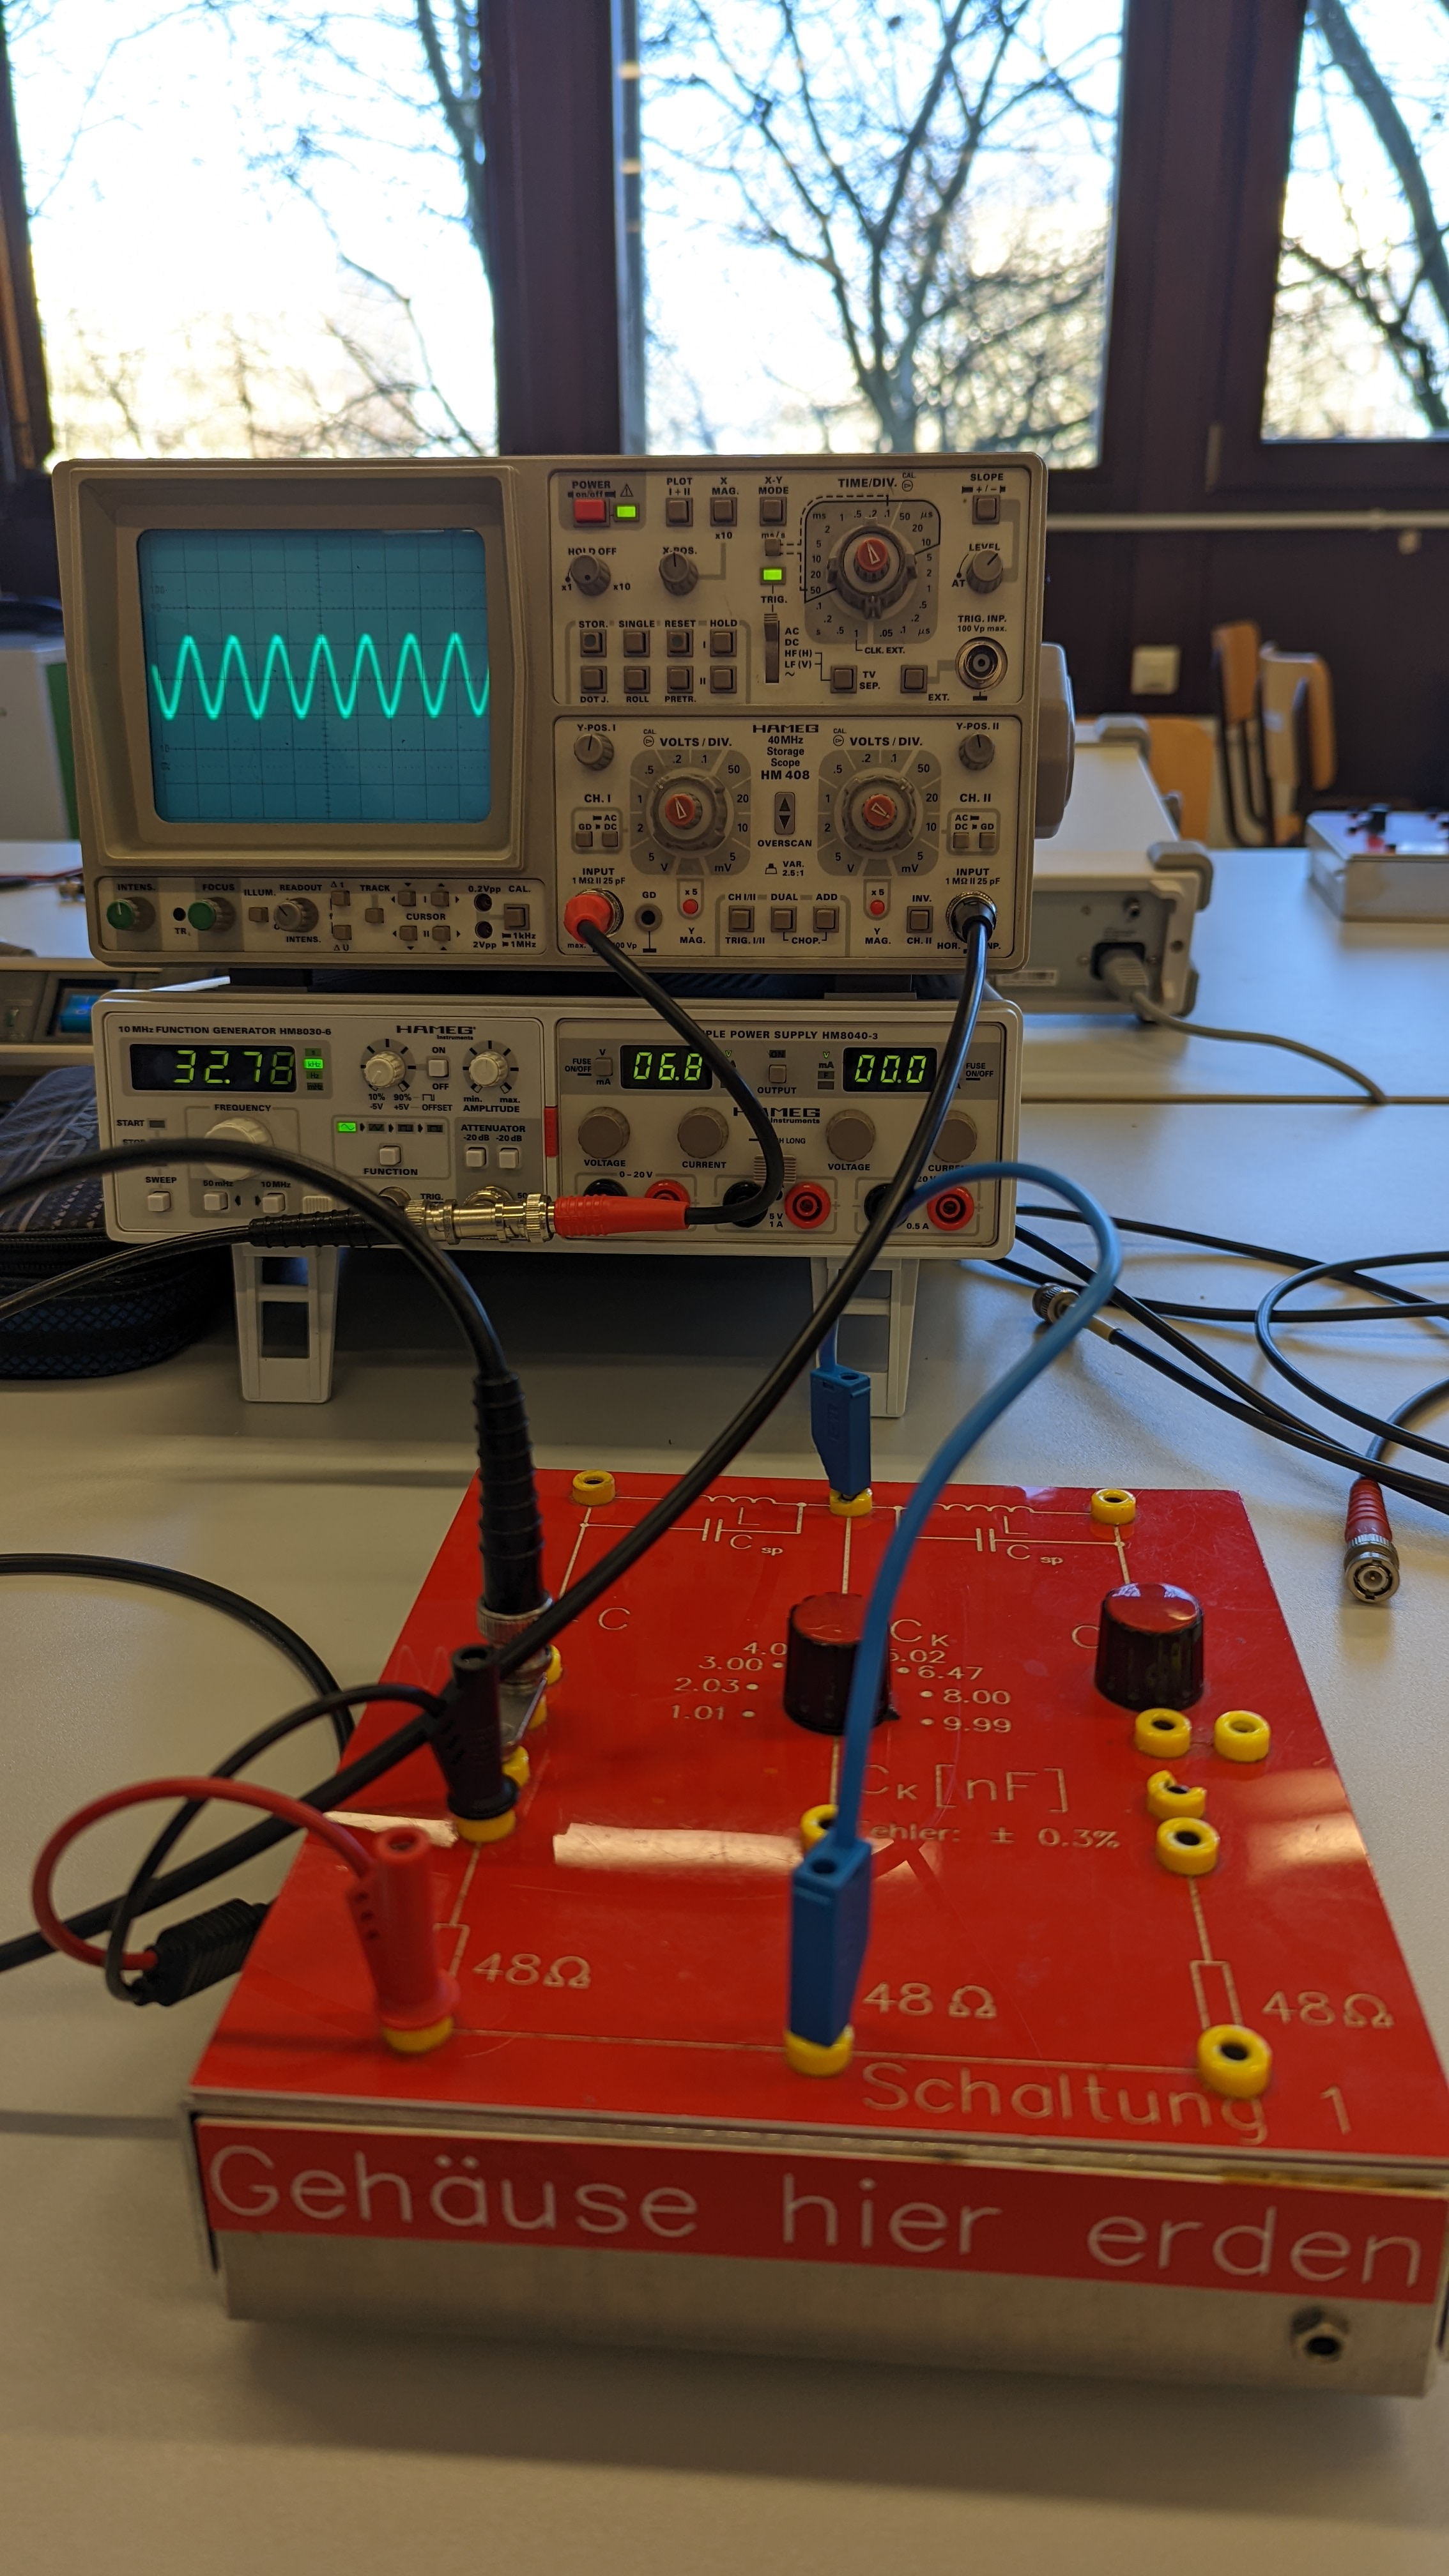
\includegraphics[width = 0.7\textwidth]{content/Aufbau1.png}
    \caption{Schematischer Versuchsaufbau des Experimentes \cite{v407}.}
    \label{fig:Aufbau1}
\end{figure}

Der drehbare Spiegel wird über einen Aufbau realisiert, welcher in \autoref{fig:Aufbau2} dargestellt ist. Der Winkel $\alpha$, welcher in \autoref{fig:Aufbau1} eingezeichnet 
ist, wird über ein \textit{Goniometer} gemessen. Bevor die Messung durchgeführt werden kann muss der gesamte Versuchsaufbau einjustiert werden, damit systematische Fehler 
ausgeschlossen werden können.  

\begin{figure}
    \centering
    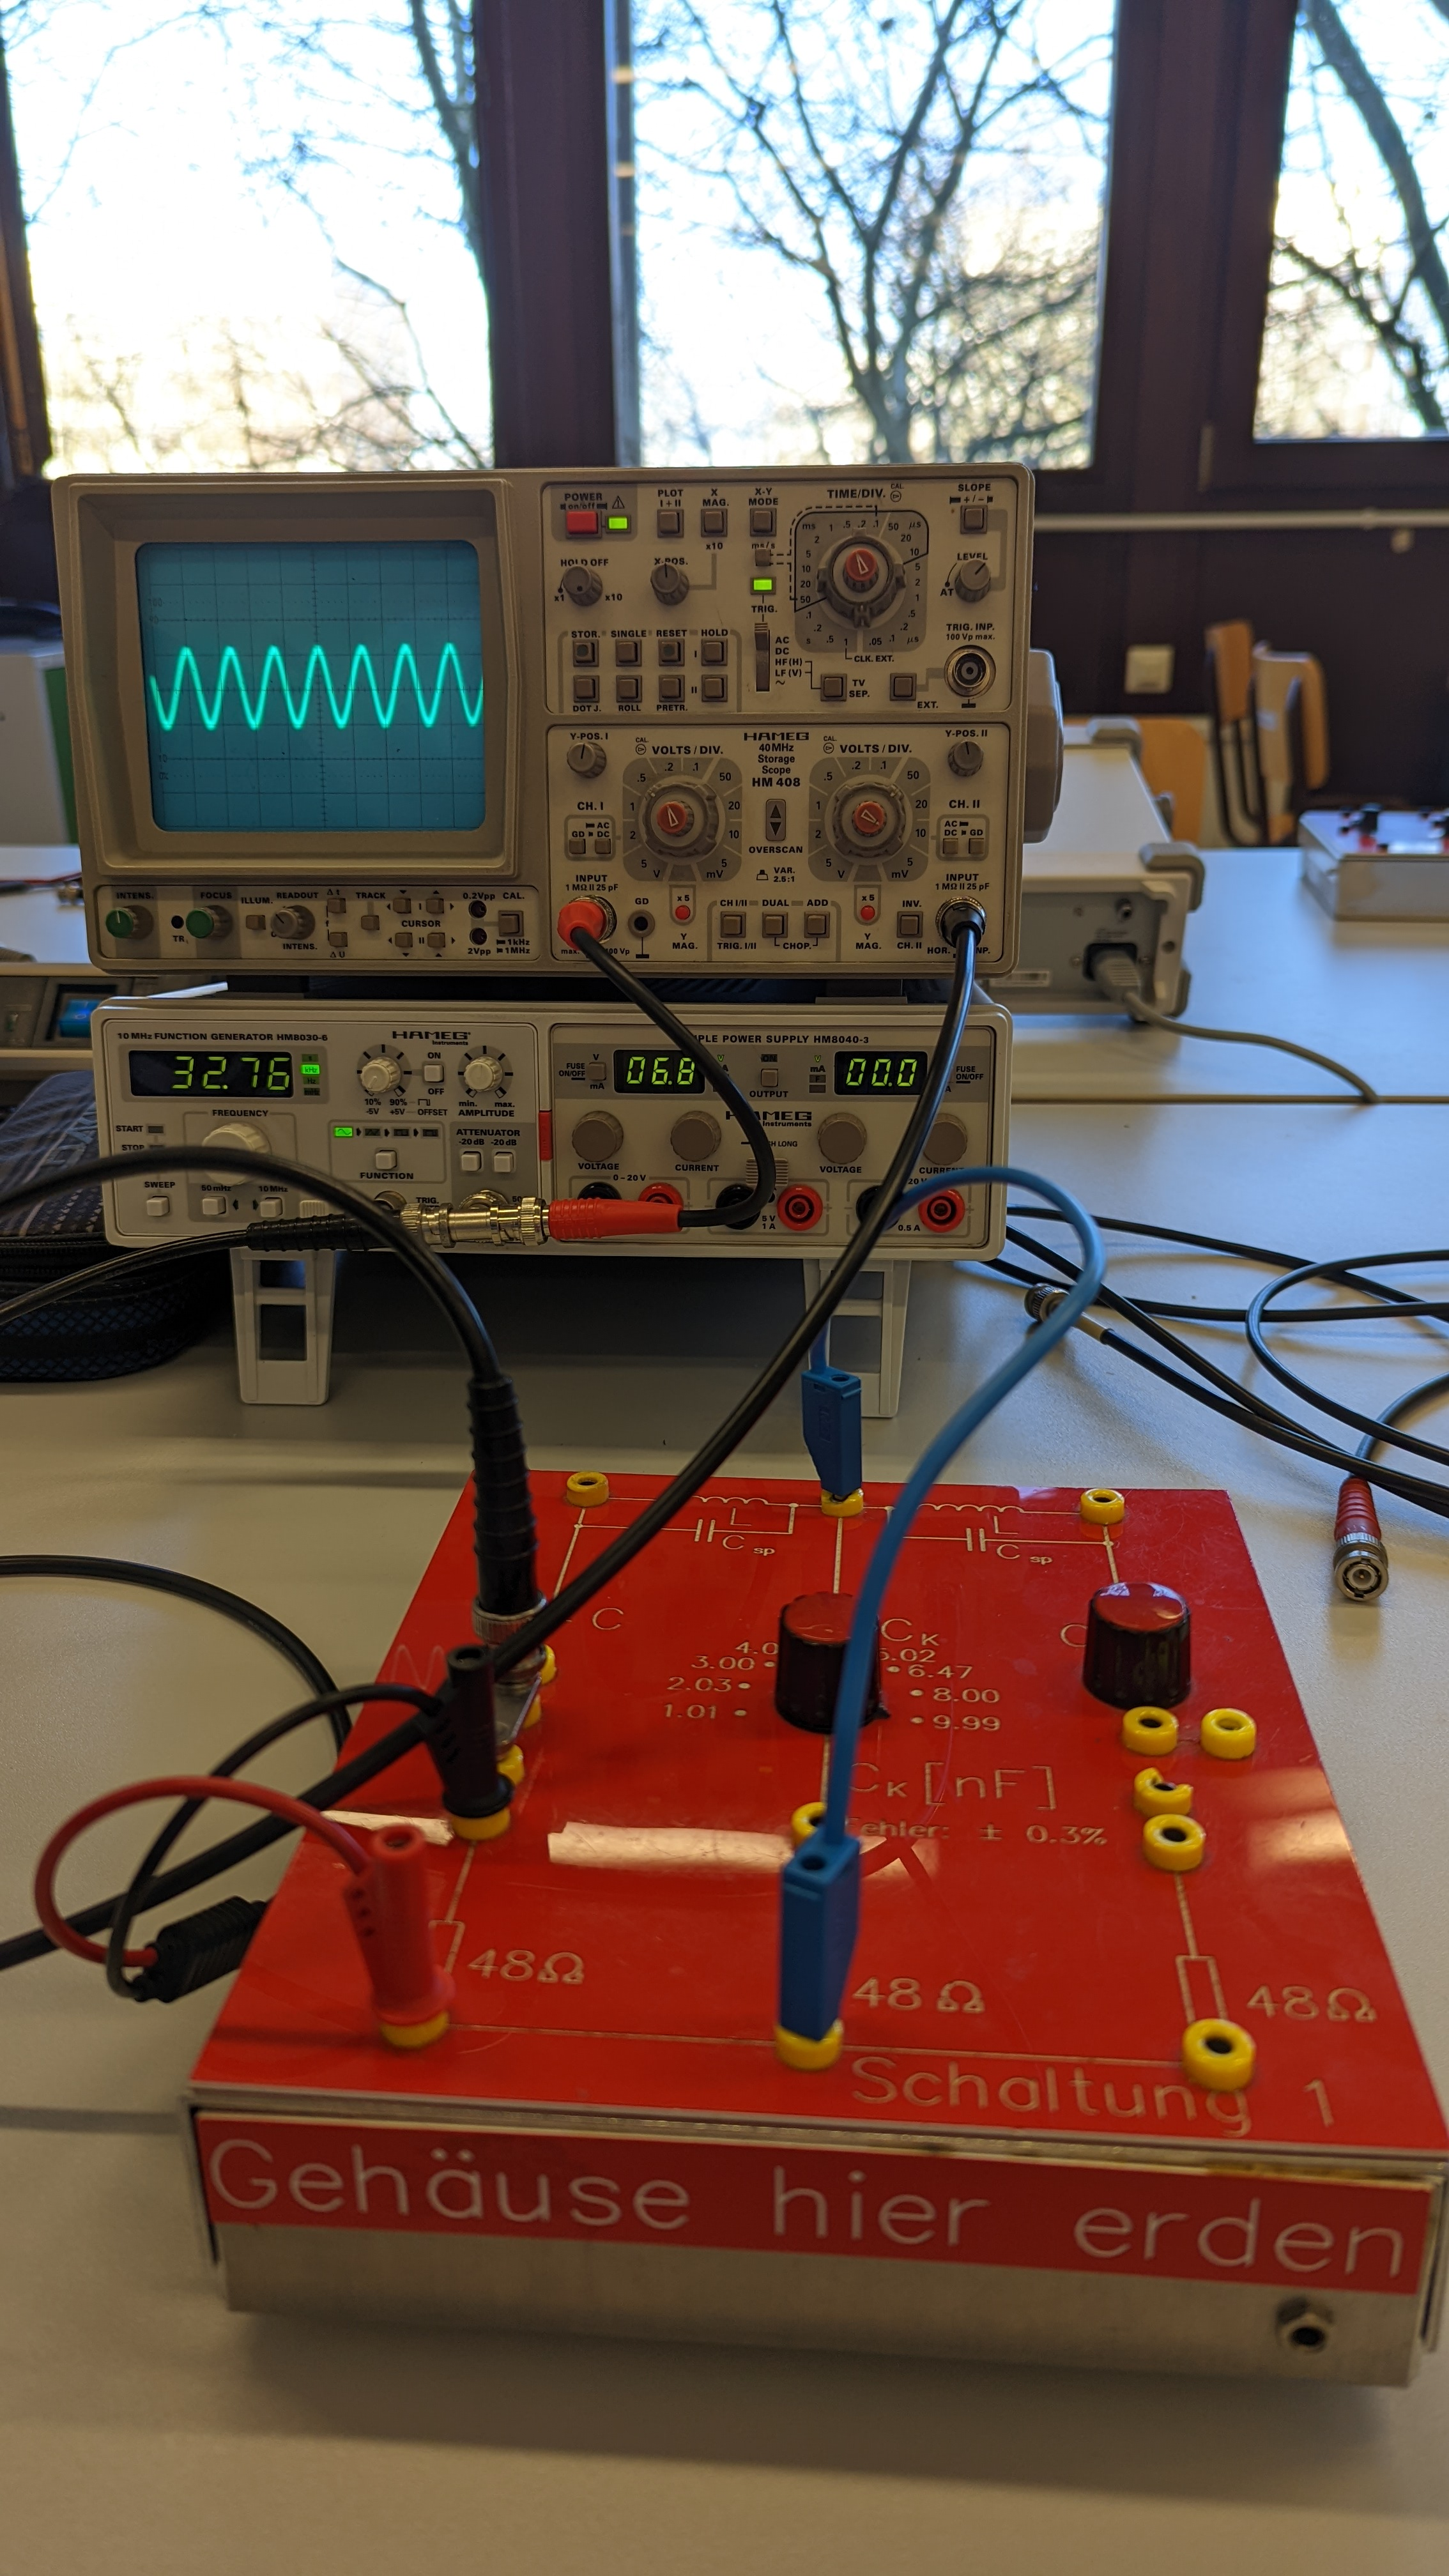
\includegraphics[width = 0.7\textwidth]{content/Aufbau2.png}
    \caption{Versuchsaufbau des Experimentes \cite{v407}.}
    \label{fig:Aufbau2}
\end{figure}

Zunächst wird der Laserstrahl auf die Goniometerachse einjustiert. Das bedeuetet, dass bei dem verwendeten Versuchsaufbau zunächst das Goniometer auf $\alpha = \qty{0}{\degree}$
eingestellt werden muss. Dann wird der Spiegel durch die entsprechende Stellschraube gelöst und gedreht, sodass der Laserstrahl so genau wie möglich in die Laseröffnung 
reflektiert wird. Dann wird die Stellschraube festgezogen. Die Höhe des Spiegels kann dabei ebenfalls durch eine in den Skizzen dargestellten Stellschrauben variiert werden.
Nach dieser Justierung ist die Apparatur messbereit. 
Bevor die Messung beginnt wird noch der Dunkelstrom des Photoelementes und  die Gesamtintensität des Laser bestimmt. Der Dunkelstrom wird bestimmt indem der Laser ausgeschaltet 
wird und dann ein Messwert an dem Amperemeter abgelesen wird. Dieser Wert entsteht durch das Umlicht und wird in der Auswertung dieses Versuches zur Korrektur verwendet. 
Die Gesamtintensität des Laser kann bestimmt werden indem der Spiegel ausgebaut wird. Dann wird das Photoelement direkt von dem p- und s-polarisierten Licht bestrahlt und 
der Messwert am Amperemeter abgelesen.

Mit der einjustierten Messapparatur werden nun Messwerte in einem Intervall von $\alpha \in \left[\qty{6}{\degree} ; \qty{88}{\degree}\right]$ aufgenommen. Dies geschieht 
jeweils zu p- und s-polarisierten Licht. Dabei wird das Messintervall in $\qty{2}{\degree}$-Schritten durchlaufen. Nach dieser Messung wird zu p-polarisiertem Licht noch eine
Detailmessung durchgeführt. Dabei werden im Bereich des Brewsterwinkels $\alpha_{\text{p}}$ genauere Winkelschritte durchlaufen. Diese Messwerte werden zu den bereits 
aufgenommenen Daten hinzugefügt.